\documentclass[12pt]{article}

\usepackage{graphicx}
\usepackage{caption}

\begin{document}

\section{Picuture \& Schema}

\begin{figure}[!htb]
	\centering
	\begin{minipage}{.5\textwidth}
		\centering
		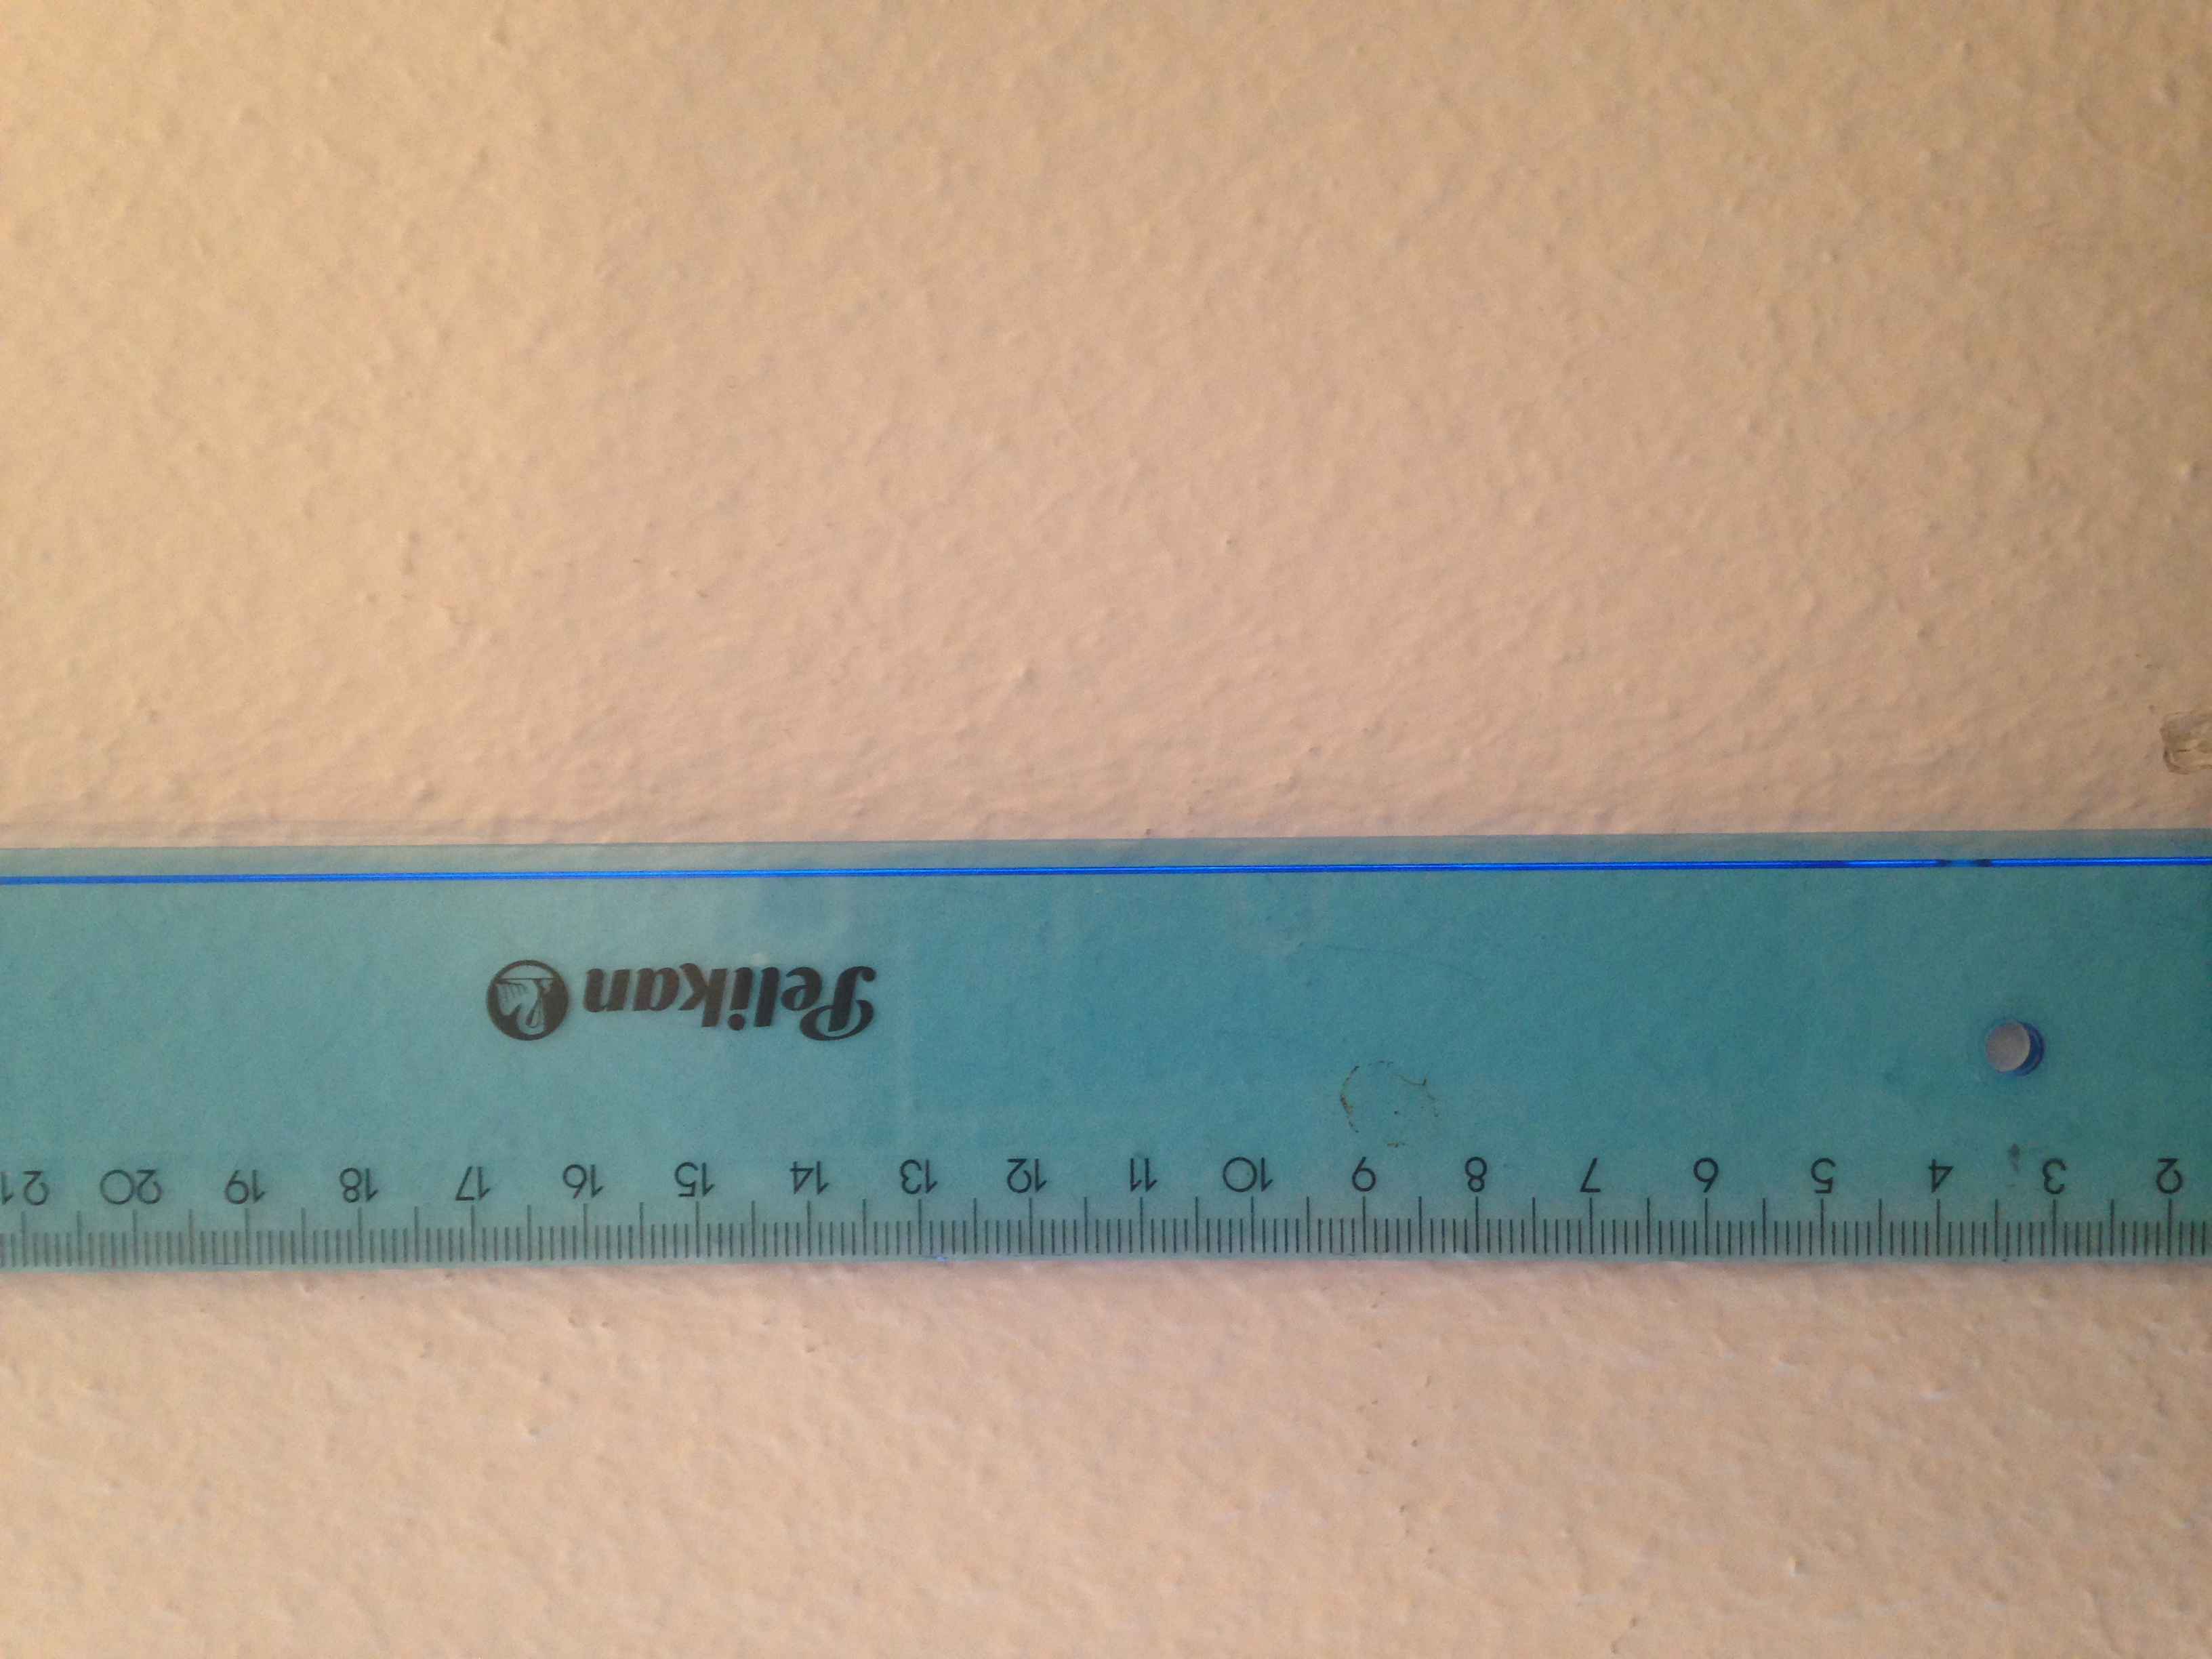
\includegraphics[width=\linewidth, angle=-90]{figures/rulerOniPhone5C}
		\captionof{figure}{Picture}
		\label{fig:Picture}
	\end{minipage}%
	\begin{minipage}{.5\textwidth}
		\centering
		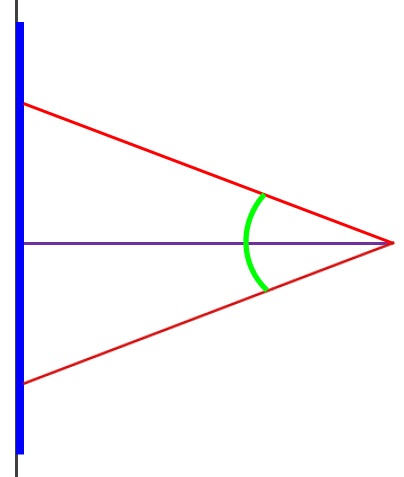
\includegraphics[width=\linewidth]{figures/schema}
		\captionof{figure}{Schema}
		\label{fig:Schema}
	\end{minipage}
\end{figure}

\section{Calculate Aspect Ration \& Field of View}

Ruler measurement top $R_{Top}=212mm$. Ruler measurement bottom  $R_{Bot}=26mm$. This yields an "in-scene" height $h$ of $212mm-26mm=186mm$. Fixed distance from the ruler to the camera $d=190mm$. We find that the vertical view angle, i.e. the field of view is $\approx\alpha=45^\circ$.
\newline\newline
Having a picture pixel size of $2448\times3264$, we calculate the aspect ratio $R=\frac{3}{4}=0.75$.
\end{document}